\chapter{Related Work}
\label{ch:related}
This chapter details existing work on vectorization and vector conversion across different image domains, specifically for the case of line art. \Cref{sec:related.vec} details works that attempt to generate a corresponding vector image given a raster image and is related to the implementation of the deep learning model for line-art vectorization as described in \Cref{sec:intro.goals} (see \gls{ro1}). \Cref{sec:crossdomain} explores cross-domain line-art vectorization, which is required for the potential extension of the model into final animation frame to clean animation frame vector conversion. While cross-domain vectorization is not the focus of this work, the goal is to design the model in a way that makes it easily adaptable for this task.

\section{Line-art Vectorization}
\label{sec:related.vec}

Since there is a non-injective relation between vector images and raster images, converting a raster image into a vector image is a non-trivial task. Hence, state-of-the-art methods primarily utilize learned models to achieve this. While there exist methods based solely on heuristic optimization \citep{Selinger03potrace:a, autotrace, 10.1145/2421636.2421640, DBLP:journals/tog/BessmeltsevS19,https://doi.org/10.1111/cgf.14485}, they do not produce the intended output for this task. As mentioned in \Cref{ch:intro}, the resulting vector primitives rarely resemble the primitives an artist would draw naturally. Crucially, these algorithms are not differentiable, meaning that they can not be finetuned to vectorize input images across domains. Additionally, they require manual hyperparameter tuning for each individual image. Furthermore, each method relies on strong assumptions on the input image, such as exceeding a specific resolution, a low signal-to-noise ratio or containing only specific junctions. Finally, and somewhat counter-intuitively, a learned method could potentially be faster, since the number of primitives in an animation line-art image is large and traditional methods have a high runtime complexity in the number of primitives. However, note that this only applies to a zero-shot model and not to the iterative deep learning models explored in this work.

While image vectorization is not yet a solved task, there have been some recent advances in deep learning for vector images. \citet{DBLP:conf/cvpr/Reddy21} introduce Im2Vec, an encoder-decoder architecture consisting of a \gls{cnn} encoder and a \gls{rnn} decoder. The \gls{cnn} encodes the image into a latent feature vector, while the \gls{rnn} is used to decode this feature vector into a fixed-length sequence of vector shapes based on multiple bezier curves. It can be trained to vectorize raster images without vector supervision (i.e., using only raster images in the ground truth training set). This would be very useful in the context of line-art vectorization. The ability to train the model without vector supervision stems from its usage of a differentiable rasterizer \citep{Li:2020:DVG}. In the general case, there are two main limitations of Im2Vec: The pixel resolution has to be defined at training time and the model does not scale well to higher resolutions. Additionally, the outputs sometimes contain degenerate features or semantically useless parts. Since clean animation line art only includes a subset of possible vector image graphic primitives, this might be avoidable by imposing (heuristic) geometric constraints.

\begin{figure}
    \centering
        \begin{tikzpicture}
    \node[draw=black] at (0,0) {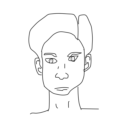
\includegraphics{graphics/im2vec/im2vec_simpletest_input_1.png}};
    \node[draw=black] at (5,0) {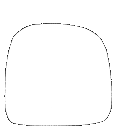
\includegraphics{graphics/im2vec/im2vec_simpletest_output_1.png}};
    \node[draw=black] at (0,5) {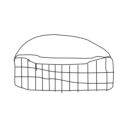
\includegraphics{graphics/im2vec/im2vec_simpletest_input_2.png}};
    \node[draw=black] at (5,5) {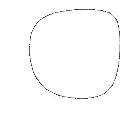
\includegraphics{graphics/im2vec/im2vec_simpletest_output_2.png}};
    \node at (0,-3) {Input};
    \node at (5,-3) {Output};
\end{tikzpicture}
    \caption{Results of Im2Vec \citep{DBLP:conf/cvpr/Reddy21} on two simple line-art sketches from \citet{eitz2012hdhso}. The image size is 128x128px.}
    \label{fig:im2vec.simpletest}
\end{figure}

However, our experiments showed that Im2Vec only works on a specific type of image, such as emojis or icons. It does not perform well when trained on line-art images, as can be seen in \Cref{fig:im2vec.simpletest}. Additionally, there were no experiments in the paper to output more than 4 shapes. It is doubtful whether it is possible to train the \gls{rnn} decoder to output the large number of bezier curves required for a clean animation frame.

The virtual sketching framework introduced by \citet{mo2021virtualsketching} is similar to Im2Vec in that it is trained without vector supervision to vectorize raster images. Other than that, it differs from Im2Vec in multiple ways. The main difference is that it constrains the output to only produce quadratic bezier curves. Also, it is an iterative model, i.e., the curves are drawn one at a time. The curves are sequentially added to a canvas in a differentiable manner. After a given number of curves is drawn, the loss is computed and propagated through all the steps. These two differences make the model more suitable for professional line art. Other differences to Im2Vec include using a different differentiable rasterizer \citep{DBLP:conf/iccv/HuangZH19a} and a finetuned perceptual loss \citep{DBLP:conf/eccv/JohnsonAF16} instead of an $L^2$ loss.
However, since the iterative model is trained mainly by computing a perceptual loss of the whole output image with the input image, the results are not semantically meaningful vector images. So while the model produces a collection of bezier curves that visually resembles the input image at a certain resolution, the vector image does not preserve the topology or meaningful structure which is necessary for clean animation frames. Related work includes ~\citet{DBLP:journals/corr/abs-2110-04830}, who use reinforcement learning as a framework for learning an iterative model in the context of comic line-art vectorization. The same constraints as with the virtual sketching framework apply here. Additionally, comic book line art does not translate well to limited animation production line art, although it would seem so at first glance.

A different approach is to incorporate parts of traditional optimization-based methods. The state-of-the-art of traditional methods was introduced by \citet{DBLP:journals/tog/BessmeltsevS19}. They attempt to detect X and T-junctions by tracing black pixel orientations with a frame field. However, additionally to the general drawbacks of traditional methods, the resulting method is not robust to more complex junctions with sharp turns, fine details or noise in general. \citet{Puhachov2021KeypointPolyvector} try to improve upon that by using a learned ensemble model to detect curve keypoints (such as junctions, start/end points and corners). Together with the input image, these keypoints are used by a geometric flow algorithm to find connections between keypoints and compute their geometry. It achieves remarkably good results, but has a more narrow aim than the proposed work. The algorithm focuses on retaining the correct stroke connectivity in the presence of noise, in their case for scanned pencil drawings. However, clean animation frames are not noisy and the curves are more narrow and densely connected, forming one large connected component for curves. Their method produces good results when applied to clean animation line art. However, resulting vector images contain overparameterized primitives and fail to vectorize more detailed and smaller shapes.

Similarly, other successful methods focus on extracting keypoints, but using a fully learned architecture. \citet{DBLP:journals/cgf/GuoZHHLW19} use a multi-task \gls{cnn} architecture to produce a centerline image and a junction image. Using this information, another \gls{cnn} extracts the curve topology. The topology image of each curve is then traced using cubic bezier least square fitting. The model is trained using raster supervision and on a synthetically created dataset. Therefore, it does not generalize well on complex real line art. Furthermore, the resulting vector image is constrained by the quality produced by the curve fitting algorithm.

On the other hand, there do exist works that attempt to fully learn a line-art vectorization model using (partially) vector supervision, which makes it easier to produce semantically meaningful vector images. \citet{DBLP:journals/tog/WangL21} use both raster and vector supervision to learn a model that generates fonts glyphs given a reference glyph. Since the number of curves required for a glyph is small ($\approx10$), the model is not trained iteratively but directly outputs a sequence of drawing commands. Their method is potentially useful, but it is doubtful whether it generalizes to a large number of curves. \citet{DBLP:journals/corr/abs-1901-03781} use solely vector supervision to reconstruct splines (which are generalizations of bezier curves). However, their approach using a hierarchical \gls{rnn} is only trained with up to three splines (with 4 to 6 control points). \citet{DBLP:conf/cvpr/BhuniaCYHXS21} use line vectorization as a self-supervised pretraining task to learn suitable sketch embeddings for downstream tasks. The line vectorization itself is similar to \citet{DBLP:conf/cvpr/Reddy21} in that it uses a \gls{cnn} as encoder and a \gls{rnn} as an encoder to generate the whole image at once. Contrary to \citet{DBLP:conf/cvpr/Reddy21} it is trained using vector supervision and constrained to output curves as a sequence of draw commands. Similar to \citet{DBLP:conf/cvpr/Reddy21}, the model is only tested with vector images containing a small number of curves.

In a similar vein, a method to generate technical drawings by \citet{DBLP:conf/eccv/EgiazarianVAVST20} is also framed as a line vectorization problem trained solely using vector supervision. It uses the Transformer architecture and is constricted to only handle 10 curves per image. To handle images with a larger amount of curves, each image is split into fixed-size tiles. The tiles are processed independently by using the Transformer model to predict vector primitives to match the curves in the image. The resulting primitives are then refined using a physics-inspired algorithm by aligning them to the black pixels in the raster image. Afterwards the primitives of all tiles are merged using a simple heuristic algorithm. While the model produces good results on technical line drawings, the authors also demonstrate that it generalizes to other line art. It is limited by the assumption that there are less than 10 curves within a tile and the reliance on the heuristic merging algorithm. The authors also show that the pure primitive predictions by the Transformer model are lacking, requiring the physics-inspired refinement algorithm, which relies on strong assumptions of the input image. This is displayed in \Cref{fig:deepvectechdraw.steps}. Additionally, the model was only tested for two vector primitives: lines and quadratic bezier curves. When applied to clean animation frames, it produces images that are both visually and structurally pretty close to the original at certain parts. However, like \citet{Puhachov2021KeypointPolyvector} it skips certain smaller and more detailed shapes. Quite paradoxically, it also produces a lot of superfluous small curves at some parts.
%Furthermore, technical line drawings do not generalize well to clean animation line art, with its more complex curves and high connectivity.

\begin{figure}
    \centering
    \begin{tikzpicture}
    \node[anchor=south west,inner sep=0] (image) at (0,0) {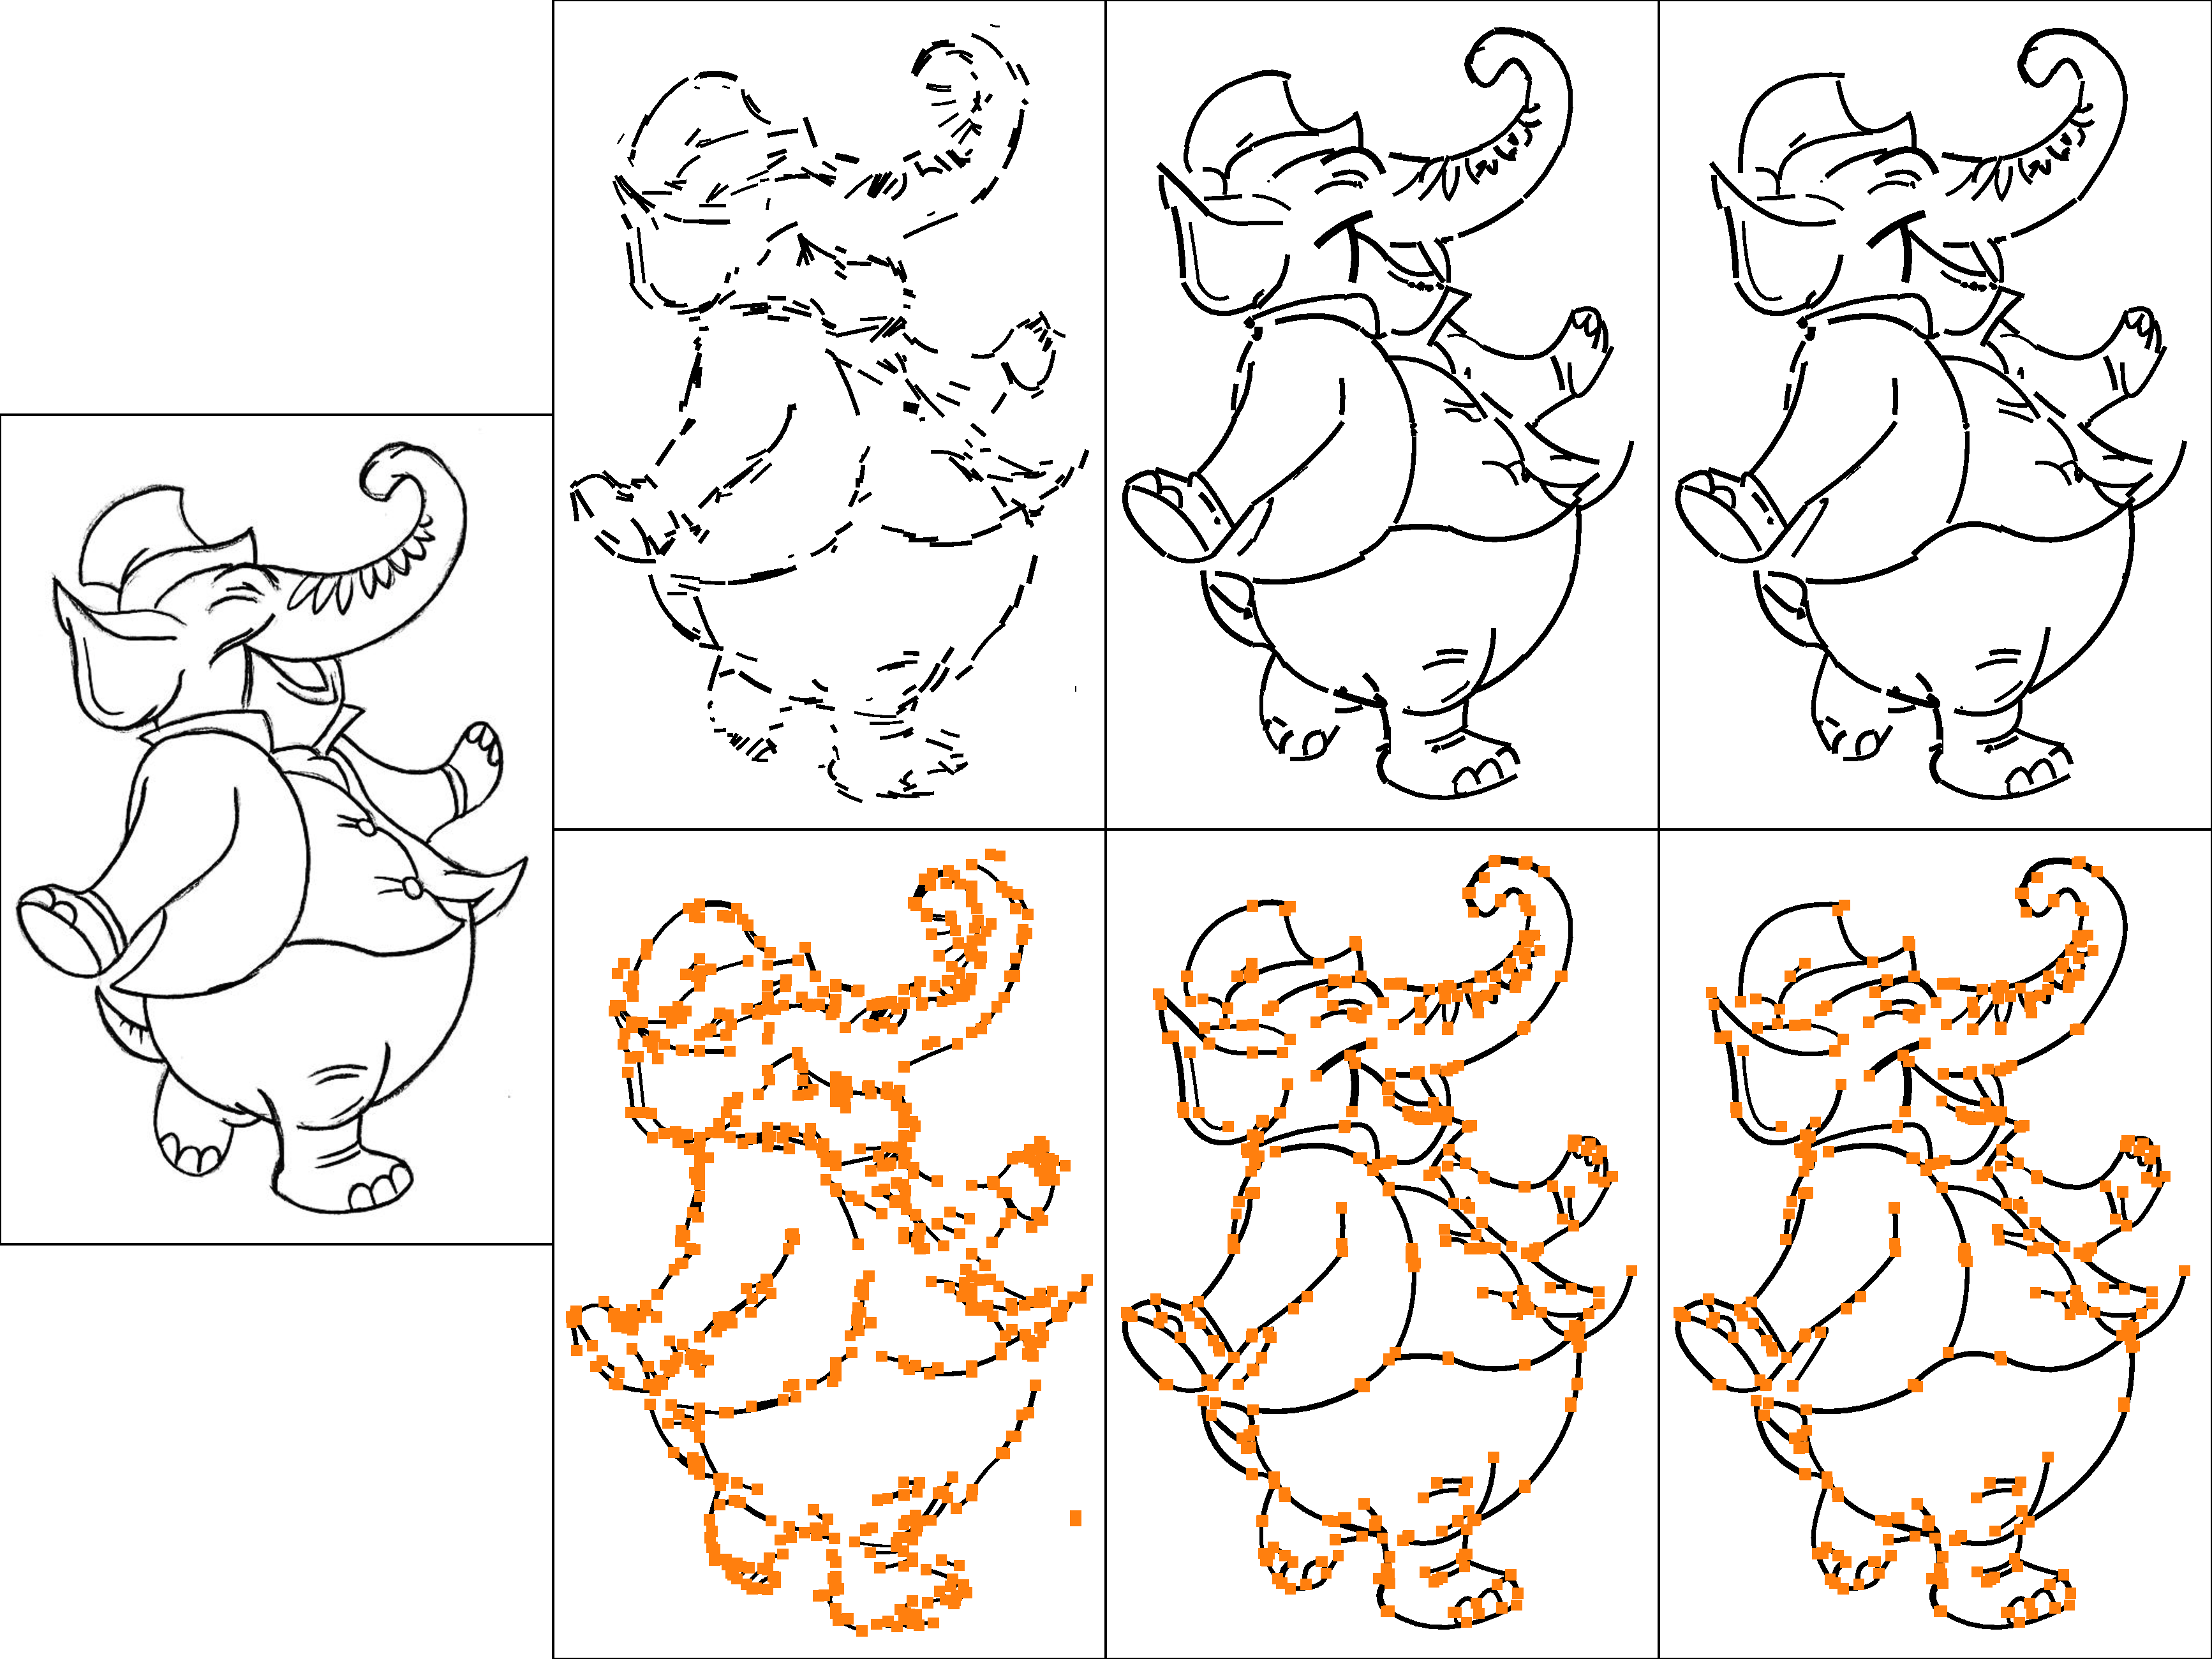
\includegraphics[width=\linewidth]{graphics/elephant.pdf}};
    \begin{scope}[x={(image.south east)},y={(image.north west)}]
        \footnotesize
        \def\y{-0.75\baselineskip}
        \def\dx{1./8}
        % Captions
        \node at (\dx,\y) [align=center] {Input};
        \node at (3*\dx, \y) [align=center] {NN};
        \node at (5*\dx, \y) [align=center] {NN + Refinement};
        \node at (7*\dx, \y) [align=center] {Full};
    \end{scope}
\end{tikzpicture}
    \caption{Result and intermediates step of the model by \citet{DBLP:conf/eccv/EgiazarianVAVST20} on line art by \citet{ivanhuska}.}
    \label{fig:deepvectechdraw.steps}
\end{figure}


\section{Cross-Domain Line-Art Vectorization}
\label{sec:crossdomain}
To our knowledge, final animation frame to clean animation frame conversion has not yet been attempted. This task is related to works attempting to generate vector line art using input images of another domain, such as photos or illustrations.

\citet{mo2021virtualsketching} provide experiments with generating vector line art using photographs as input. However, the authors concede that the model does not generalize well to complex images and produces artifacts.

The model proposed by \citet{Puhachov2021KeypointPolyvector} can be regarded as the state-of-the-art for sketch to clean vector line image conversion. However, the method relies on strong assumptions regarding the input image, specifically regarding the background-foreground threshold, which prevents the method to be used for drawings with a very noisy background (such as final animation frames).

\citet{LIPS2019} implement a GAN to generate raster contour sketch images given realistic photos as input. It is doubtful whether the results produced by this method would lead to a semantically meaningful vector image. Either way, \citet{mo2021virtualsketching} seem to outperform this method (and produce cleaner results due to the fact that the output is restricted to vector primitives).

There exists related work specifically related to anime-style illustrations. \citep{sketch} devise a model which produces a raster line art given an illustration. The results contain substantial artifacts and are therefore not quite usable as clean animation line art. The two main problems are lack of high quality training data and pixel-level supervision. The colored-sketch pair dataset normally used for such models \citep{pixiv} only superficially resembles clean animation frames, primarily since the line-art images have variable stroke widths.

\citet{Manga2021zhang} generate manga-style images from illustrations. The generation is constrained by the actual manga creation workflow. The first step of this workflow is the generation of line art given the illustration using a U-Net architecture \citep{DBLP:conf/miccai/RonnebergerFB15}. This could be used to generate a raster line art given a final animation frame. Then, the raster image could be vectorized using the line-art vectorization model. Unfortunately, the data used to train this model is not public. Furthermore, the provided results contain artifacts which will likely make it challenging to correctly vectorize the image.